
The following is an account of activity within the CSC DPG carried out by the contact to the AlCaDB group and by the CSC Validation team during the time period from late 2018 to the present. For conditions-related work, this covers the studies and validation performed on new calibration constants and timing corrections, updates to bad chambers conditions, and any new payloads uploaded to the conditions database. A description of CSC Validation, a function of the CSC DPG, is also provided along with a brief account of software development required during the same time period.

\subsection{Contact to AlCaDB}

Immediately following the conclusion of LHC Run II, CSC operations performed several calibration runs (325875, 325656, and 325875). The ``new'' calibration constants were extracted from run 325875 with \texttt{CMSSW\_10\_2\_11}. These were compared to ``old'' constants already in the conditions database under the Express tags: \texttt{CSCDBPedestals\_express}, \texttt{CSCDBGains\_express}, \texttt{CSCDBNoiseMatrix\_express}, and \texttt{CSCDBCrosstalk\_v2\_express}, each with an IOV of run 266576. Figures x-x show the relative differences in each cathode channel between the new constants and the old. Validation of the new conditions data on reconstruction is necessary to determine if the conditions are fit to upload. Using RAW SingleMuon data from Run 2018D, events were reconstructed using the old and new conditions data separately. Validation plots showing the rechit-to-segment residuals in layer 3 of the CSCs ring ME1/1 are shown in Figs.~\ref{fig:CalibVal1}. These studies were presented to the CSC experts (including the CSC DPG) in the CSC weekly meeting on April 17, 2019. The conclusion was drawn that the constants were stable and did not need replacing in the conditions database. 

\begin{figure}[H]
    \centering
    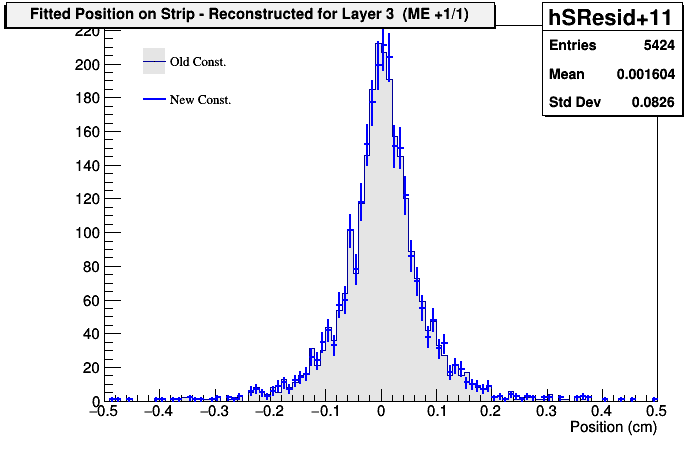
\includegraphics[width=0.49\textwidth]{Images/DetectorPerformance/CSCCalibStudy2019/ConstValidationPlots/hSResidplus11.png}
    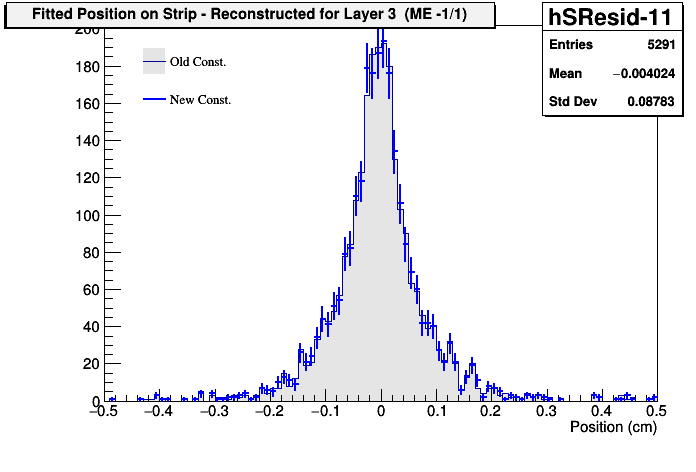
\includegraphics[width=0.49\textwidth]{Images/DetectorPerformance/CSCCalibStudy2019/ConstValidationPlots/hSResidminus11.png}
    \caption{Rechit-to-segment residuals in layer 3 of ME1/1 chambers in RAW SingleMuon 2018D data using newly-derived calibration constants in Run 2. Left: Chambers in the positive muon endcap. Right: Chambers in the negative muon endcap.}
    \label{fig:CalibVal1}
\end{figure}

With the LHC shutdown and chambers extracted for LS2, no updates to the conditions data were necissary. However, a campaign by AlCaDB to test run-dependant conditions resulting from needs by other CMS detctors required attention from the CSC DPG contact. Mock conditions were prepared to mimic a dead chamber. This was uploaded to the conditions database for AlCaDB to test the new run-dependant workflow.

It is important to make sure CSC conditions data in the conditions database reflect the state of the detector, especially before starting a new data-taking period, a MC or ReReco campaign, or when significant changes to the CSCs are made. The replacement of cathode front-end electronics on all CSCs in Ring 1 during LS2 meant new calibrations and timing corrections had to be studied. In fall of 2022, shortly after the LHC resumed collisions at \SI{13}{TeV} for Run 3, CSC Operations performed a number of calibration runs. New calibration constants were extracted from these runs with \texttt{CMSSW\_12\_0\_4} and were compared to old constants currently in the conditions database under the HLT tags: \texttt{CSCDBPedestals\_hlt}, \texttt{CSCDBGains\_hlt}, \texttt{CSCDBNoiseMatrix\_hlt}, and \texttt{CSCDBCrosstalk\_v2\_hlt}, each with an IOV of run 266566. The relative differences between the new constants and the old in each cathode channel were found to vary only slightly, mostly in the channels of chambers refurbished in LS2. The new constants were validated using Run 357735 from the RAW Muon 2022D-v1 dataset. Old calibrations for used in processing the data for validation were under the GT \texttt{124X\_dataRun3\_v9}, and the Offline tags \texttt{CSCDBPedestals\_v2\_offline}, \texttt{CSCDBGains\_v2\_offline}, \texttt{CSCDBNoiseMatrix\_v2\_offline}, and \texttt{CSCDBCrosstalk\_v2\_offline}, each with an IOV of 232000. The validation was performed using \texttt{CMSSW\_12\_4\_6}. Figure~\ref{fig:CalibVal2} show validation plots comparing the effect on the rechit-to-segment residuals when using the old and new calibrations constants in layer 3 of ME+3/1 chambers. Initially, poor position resolution in the ME1/1A chambers (ME1/1 strips were ganged into groups ``A'' and ``B'' for Run 1, but were unganged during Run 2) was observed in data reconstructed with the new constants. However, after replacing all the new calibrations constants in these channels with old constants, and reperforming the validation, the poor resolution persisted, shown in Fig.~\ref{fig:CalibVal2ME11A} Good hit resolution seen in CSC DQM with the old constants confirms that the poor resolution in validation is not a result of the conditions data used in reconstruction, but some issue with the validation code. Work identifying and resolving the issue is underway.

\begin{figure}[H]
    \centering
    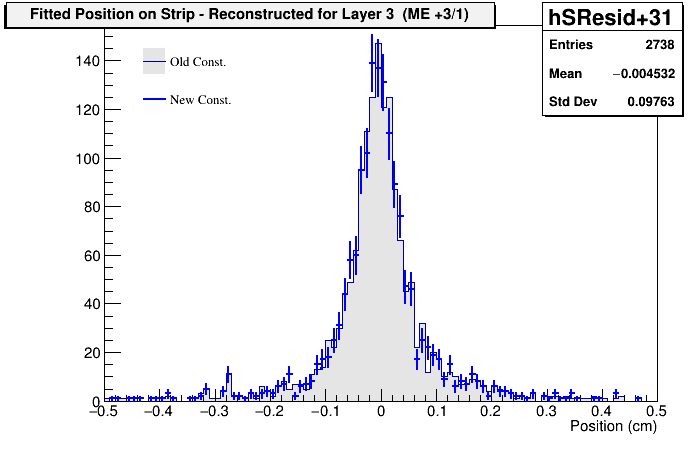
\includegraphics[width=0.49\textwidth]{Images/DetectorPerformance/run_10000012_oldME11A/hSResidplus31.png}
    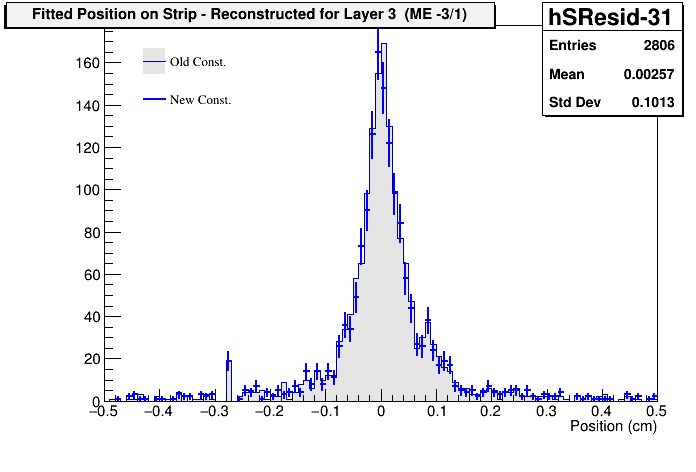
\includegraphics[width=0.49\textwidth]{Images/DetectorPerformance/run_10000012_oldME11A/hSResidminus31.png}
    \caption{Rechit-to-segment residuals in layer 3 of ME3/1 chambers in Run 357735 of the RAW Muon 2022D-v1 dataset using newly-derived calibration constants in Run 3. Left: Chambers in the positive muon endcap. Right: Chambers in the negative muon endcap.}
    \label{fig:CalibVal2}
\end{figure}

\begin{figure}[H]
    \centering
    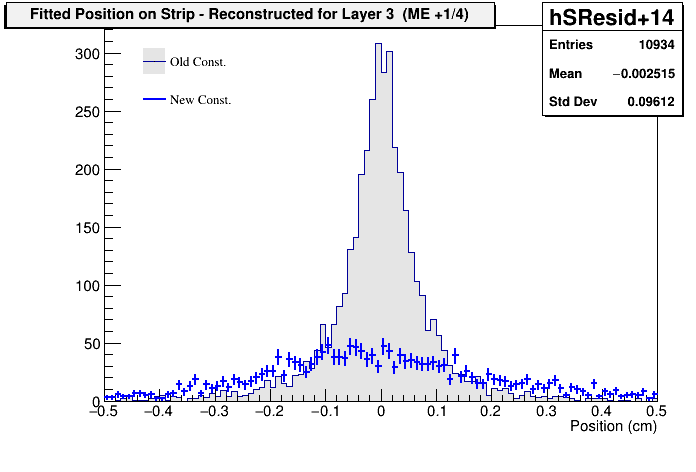
\includegraphics[width=0.49\textwidth]{Images/DetectorPerformance/run_10000012_oldME11A/hSResidplus14.png}
    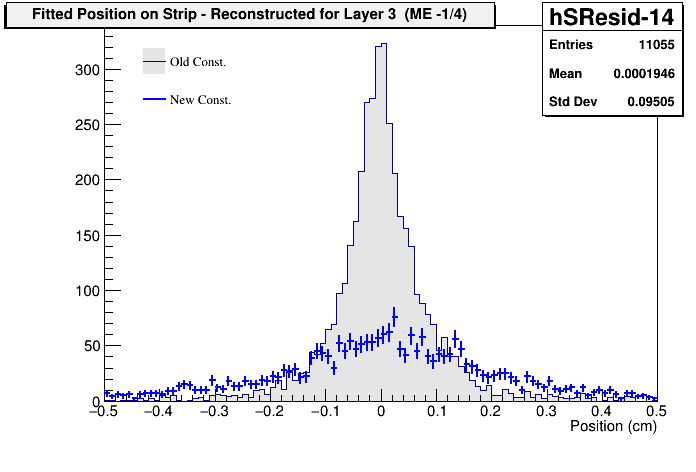
\includegraphics[width=0.49\textwidth]{Images/DetectorPerformance/run_10000012_oldME11A/hSResidminus14.png}
    \caption{Rechit-to-segment residuals in layer 3 of ME1/1A (labeled ME$\pm$1/4) chambers in Run 357735 of the RAW Muon 2022D-v1 dataset using old calibration constants extracted in Run 2. Left: Chambers in the positive muon endcap. Right: Chambers in the negative muon endcap.}
    \label{fig:CalibVal2ME11A}
\end{figure}

Split-peaks were observed in ME234/1 (chambers refurbished in LS2) cathode rechit and segment times with early Run 3 data, when reconstructed with the timing corrections derived in Run 2, as shown for ME+2/1 CSCs in Fig.~\ref{fig:TimingVal1}. New timing constants were derived with Run 357900 in the Muon 2022D dataset. The constants were checked and found not to vary in 2022. The constants were validated with the same run in the RAW Muon dataset from 2022D. Use of the new timing constants in Run 3 data greatly improved the cathode rechit and segment times, as shown in Fig.~\ref{fig:TimingVal1}. The new constants were uploaded to the conditions database, first for the Offline stream, ahead of the ReReco campaign of 2022A-E data: 
\begin{itemize}
    \item GT: \texttt{124X\_dataRun3}
    \item Record: \texttt{CSCChamberTimeCorrections}
    \item Tag: \texttt{CSCChamberTimeCorrections\_v3\_offline}
    \item IOV: 347750
    \item Insertion time: 10/10/2022
\end{itemize}

Following a Fast-Track validation by the AlCaDB group of the Express/Prompt/HLT tags with a RAW Muon 2022E-v1 dataset (Run 359699) the constants were uploaded for real data taking:
\begin{itemize}
    \item GT: \texttt{124X\_dataRun3\_[Prompt/Express/HLT]}
    \item Record: \texttt{CSCChamberTimeCorrections}
    \item Tag: \texttt{CSCChamberTimeCorrections\_hlt}
    \item IOV: 361040
    \item Insertion time: 24/10/2022 
\end{itemize}

\begin{figure}[H]
    \centering
    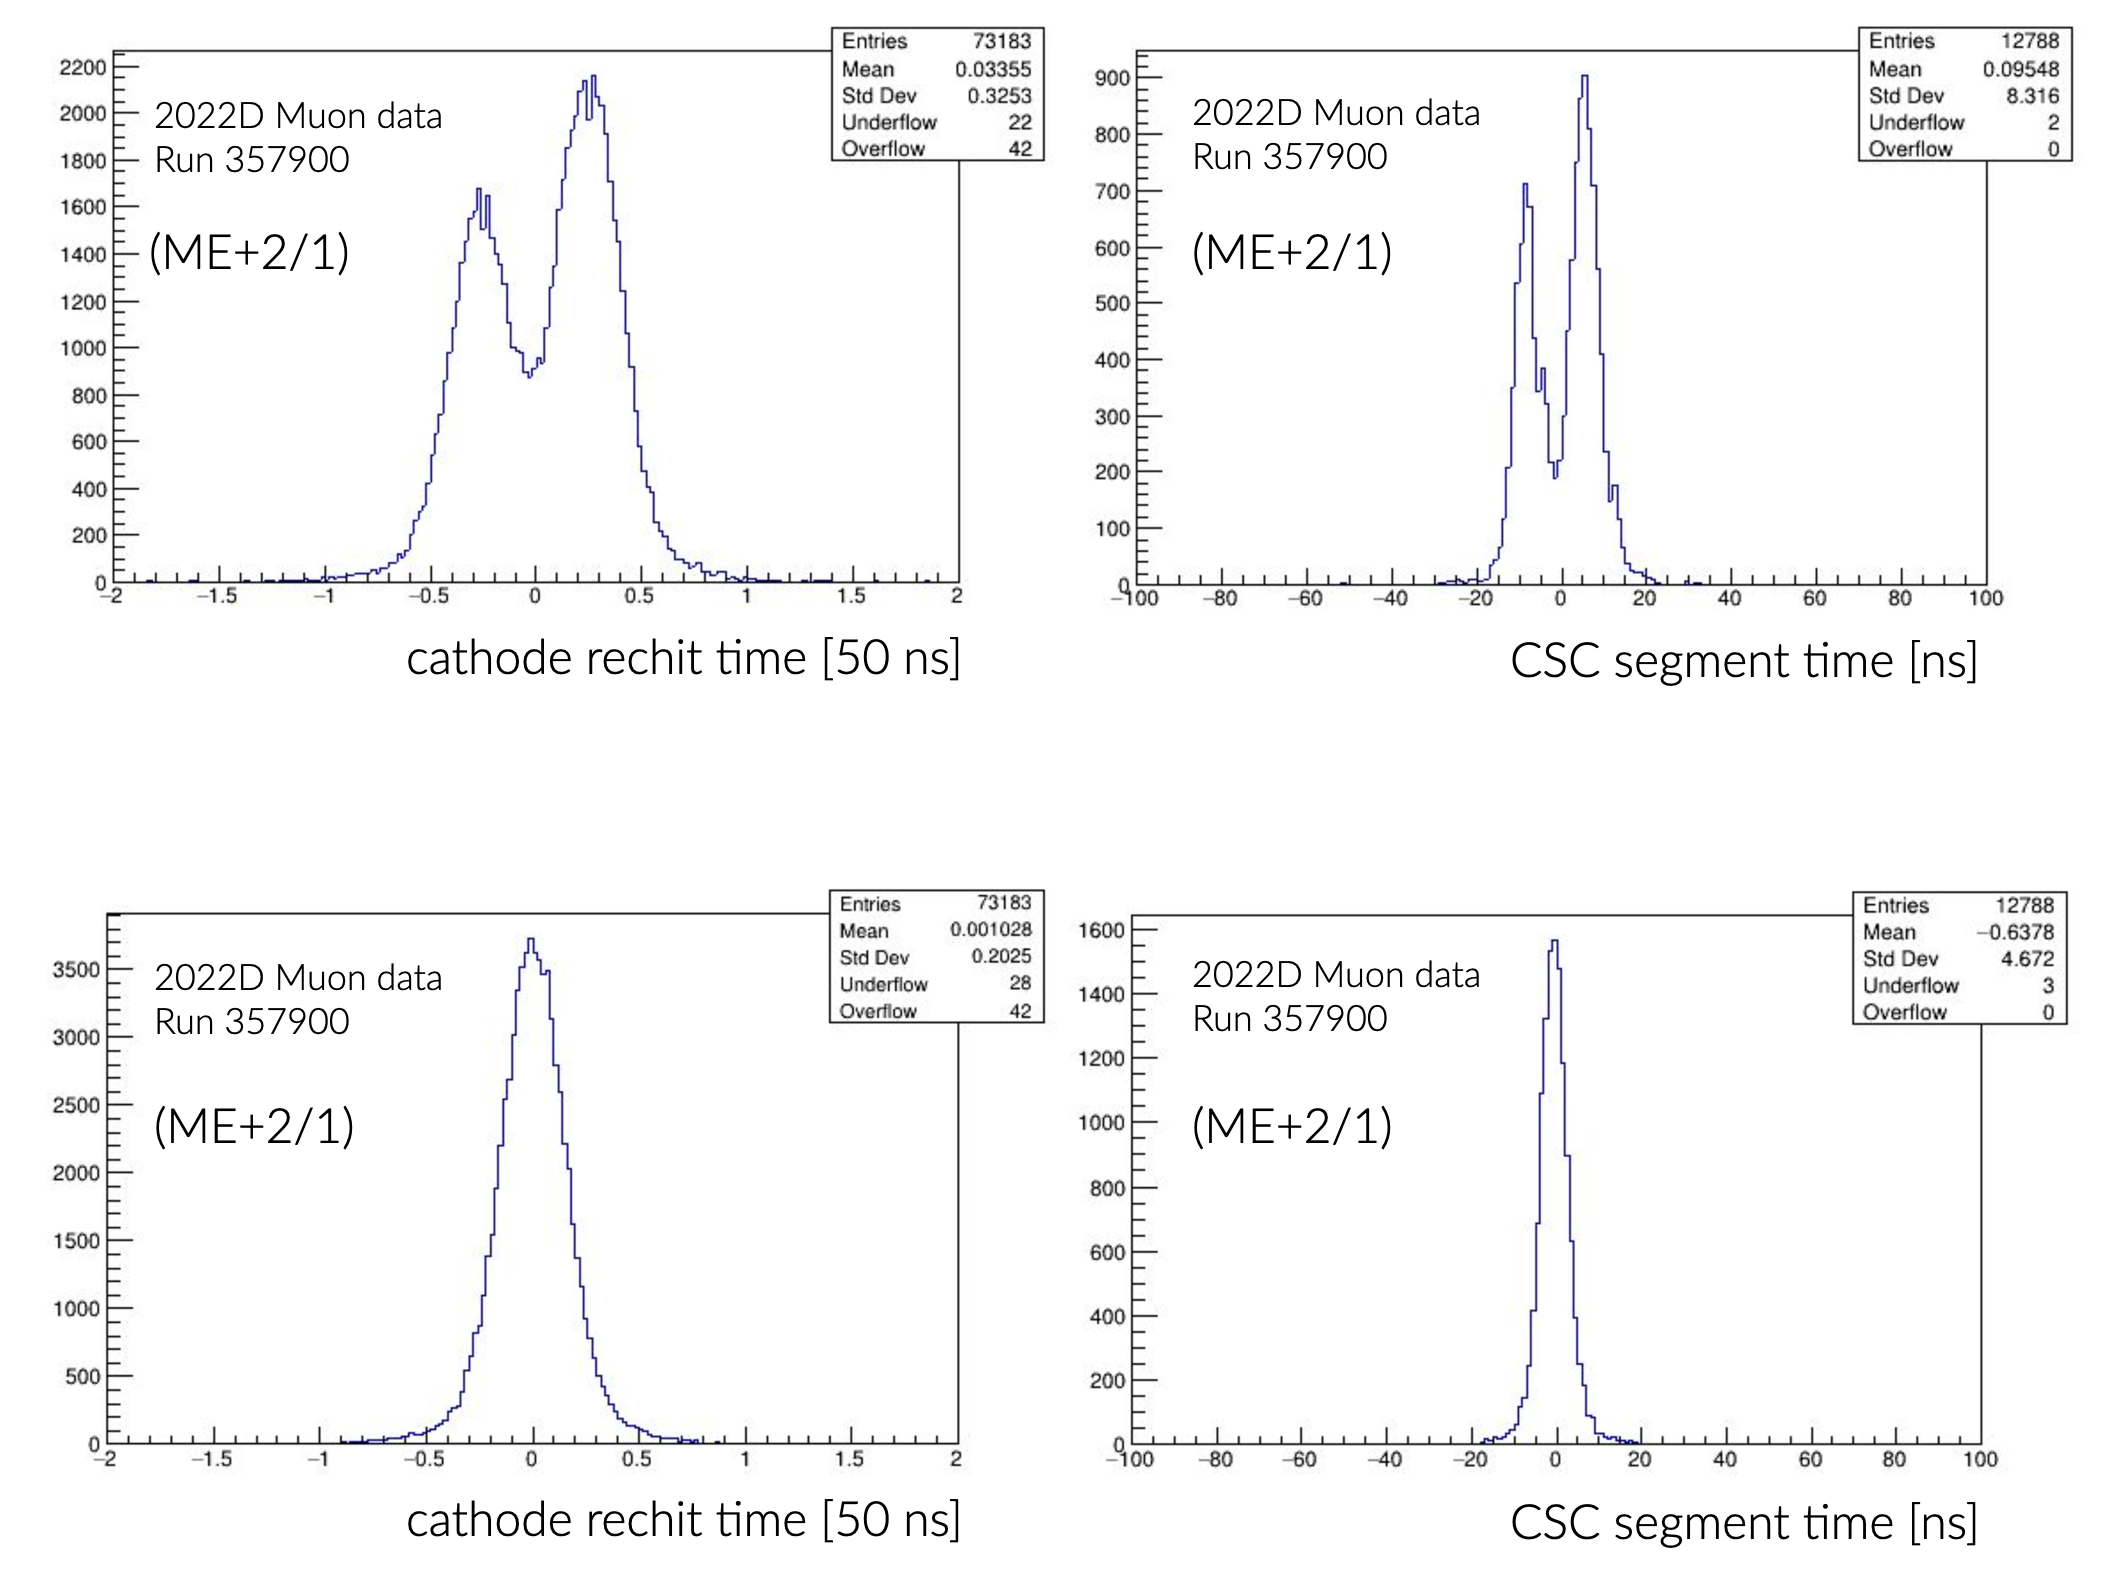
\includegraphics[width=1\textwidth]{Images/DetectorPerformance/TimingStudy/CSCRechitSegmentTimes.png}
    \caption{Top-left: Cathode rechit times using Run 2 timing corrections. Top-right: CSC segment times using Run 2 corrections. Bottom-left: Cathode rechit times using Run 3 timing corrections. Bottom-right: CSC segment time using Run 3 timing corrections. All times are for ME+2/1 chambers in RAW Muon data from Run 2022D. Left: Chambers in the positive muon endcap. Right: Chambers in the negative muon endcap.}
    \label{fig:TimingVal1}
\end{figure}

AlCaDB workshops are held annually. These workshops are designed to allow each subsystem to share the current status and plans for their conditions and alignment. It also serves as an opportunity for AlCaDB to review news, upcoming campaigns, and host tutorials for common tools. The CSC DPG contact to AlCaDB always prepares an oral presentation outlining what conditions data are used by CSCs, the current status of conditions data in offline, HLT/Express/Prompt, and MC streams, and any plans to update the conditions data.

\subsection{CSC Validation}

During normal CSC operation, it is important to verify the status of detector-components. An automated procedure called CSC Validation generates simple plots (similar to CSC DQM plots) and posts them to the CSC Valdiation website to be monitored. A software package called auto-validation submits lxplus batch jobs via a cron daemon that run the CSC Validation code producing the validation plots. Data consumed are usually RAW Muon files from Express and PromptReco runs. The auto-validation software is mostly self-contained; human intervention is rarely needed. Even so, a support team within the CSC DPG is tasked with the maintainance and development of CSC Validation. A familiarity with the workflow by the CSC Validation team esures the success of occasional special tasks or deployment of new features, in cases when external modules depreciate or centralized services like lxplus batch get phased out. 

The HTCondor software suite offers users on CERN lxplus machines acces to a High-Throughput Computing (HTC) environment. This allows the shared computing resources in CERN's machine network to be used fairly and efficiently for all users. When a user submits jobs to HTCondor on lxplus, the jobs are placed in a queue. Parameters such as number of CPUs requested, expected job duration, quantity of jobs, share of resources alloted to different experiments, and a user's priority score, impact queue placement. Once at the front of the queue, a job is sent to an availible worker node on the distributed computing service to be run. If a machine crashes or is otherwise unavailible, HTCondor will automatically restart the job on a free machine. This is essential when running thousands of jobs with on numerous datasets. When a job finishes running, the output and any errors are returned to the user. During the author's tenure on the CSC Validation team, he migrated the auto-validation code from submitting jobs via lxplus batch to submitting jobs via HTCondor. 